\documentclass[english]{article}
\usepackage{lmodern}
\usepackage[T1]{fontenc}

\usepackage{geometry}
\geometry{verbose,tmargin=3cm,bmargin=3cm,lmargin=2.5cm,rmargin=2.5cm}
\usepackage{textcomp}
\usepackage{amstext}
\usepackage{graphicx}
\usepackage{amsmath}
\graphicspath{ {./Figures/} }
\makeatletter


\providecommand{\tabularnewline}{\\}

\makeatother

\usepackage{babel}
\begin{document}

\title{3F8: Inference\\
 Short Lab Report}

\author{Yongqing Jiang}
\maketitle
\begin{abstract}
Binary classification is the foundation supervised 
machine learning. 
This study investigates binary classification on a 
non-linearly separable dataset using 
Maximum Likelihood Estimation (MLE)
to apply both linear and non-linear Gaussian 
Radial Basis Functions (RBF)
classifier. While the linear model 
provides a limited accuracy, 
the RBF method significantly improves performance, 
achieving an 82\% test accuracy through
parameter selection. The results demonstrate 
that non-linear basis functions are essential 
for capturing complex decision boundaries and 
achieving better model generalization.

\end{abstract}

\section{Introduction}
In this lab activity, we design and implement a 
binary classifier using MLE to 
optimize the parameter  $\beta$. 
The dataset presents a significant 
challenge due to its non-linearly 
separable distribution.
 
The performance of linear model and RBF method 
is rigorously assessed using the 
final average log-likelihood values 
and confusion matrices, providing 
insights into the trade-off between 
model complexity and generalization.

\section{Exercise a)\label{sec:Exercise-a}}

In this exercise we have to consider the logistic classication model
(aka logistic regression) and derive the gradients of the log-likelihood
given a vector of binary labels $\mathbf{y}$ and a matrix of input
features $\mathbf{X}$. The gradient of the log-likelihood can be
writen as
\begin{equation*}
   \frac{\partial\mathcal{L}(\beta)}{\partial\beta}=
   \sum_{n=1}^{N} (y^{(n)} - \sigma(\beta^T \tilde{x}^{(n)}))\tilde{x}^{(n)}
   = \tilde{\mathbf{X}} (\mathbf{y} - \sigma(\tilde{\mathbf{X}}\beta ))
\end{equation*}




\section{Exercise b)}

In this exercise we are asked to write pseudocode to estimate the
parameters $\beta$ using gradient ascent of the log-likelihood. Our
code should be vectorised. The pseudocode to estimate the parameters
$\beta$ is shown below:
\begin{verbatim}
Function estimate_parameters:

   Input:  feature matrix X, labels y
   Output: vector of coefficients b
	
   Code:
      for i from 0 to step_num begin
         sigmoid_val = sigmoid(X, beta)
         b = b + alpha * (X(y - sigmoid_val))
         end 
      return b
\end{verbatim}
The learning rate parameter $\eta$ is chosen to be $10^{-3}$.

\section{Exercise c)}

In this exercise we visualise the dataset in the two-dimensional input
space displaying each datapoint's class label. The dataset is visualised
in Figure \ref{fig:data_visualisation}. By analising Figure \ref{fig:data_visualisation},
we conclude that a linear classifier is not applicable on this 
problem. This distribution of class 1 and class 2 is clearly 
linearly inseparable as it has a non-linear class boundary.

\begin{figure}
\begin{centering}

\includegraphics[width=0.3\paperwidth]{fig1.png}
\par\end{centering}
\caption{Visualisation of the data.\label{fig:data_visualisation} }
\end{figure}


\section{Exercise d)}

In this exercise we split the data randomly into training and test
sets with 800 and 200 data points, respectively. The pseudocode from
exercise a) is transformed into python code as follows:
\begin{verbatim}
def fit_w(X_tilde_train, y_train, X_tilde_test, y_test, n_steps, alpha):
   w = np.random.randn(X_tilde_train.shape[ 1 ])
   ll_train = np.zeros(n_steps)
   ll_test = np.zeros(n_steps)
   for i in range(n_steps):
       sigmoid_value = predict(X_tilde_train, w)
       w += alpha * (X_tilde_train.T@(y_train - sigmoid_value))
       ll_train[ i ] = compute_average_ll(X_tilde_train, y_train, w)
       ll_test[ i ] = compute_average_ll(X_tilde_test, y_test, w)
   return w, ll_train, ll_test
\end{verbatim}
We then train the classifier using this code. We fixed the learning
rate parameter to be $\eta=10^{-3}$ . The average log-likelihood on the
training and test sets as the optimisation proceeds are shown in Figure
\ref{fig:learning_curves}. By looking at these plots we conclude
that this model converges and it has a reasonable learning rate.


Figure \ref{fig:learning_curves} displays the visualisation of the
contours of the class predictive probabilities on top of the data.
This figure shows that our intuition about the limit of a linear classifier
was correct. This classification can not be achieved by linear classifier. 
Non-linear terms should be used to classify.

\begin{figure}
\begin{centering}

\includegraphics[width=0.3\paperwidth]{fig2.png}\hspace{1cm}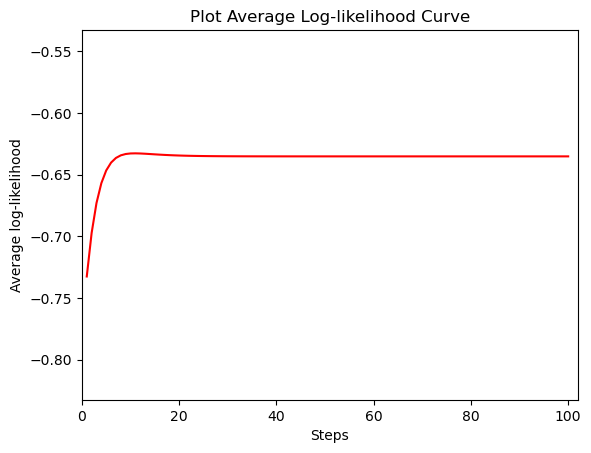
\includegraphics[width=0.3\paperwidth]{fig3.png}
\par\end{centering}
\caption{Learning curves showing the average log-likelihood on the training
(left) and test (right) datasets.\label{fig:learning_curves} }
\end{figure}

\begin{figure}
\begin{centering}
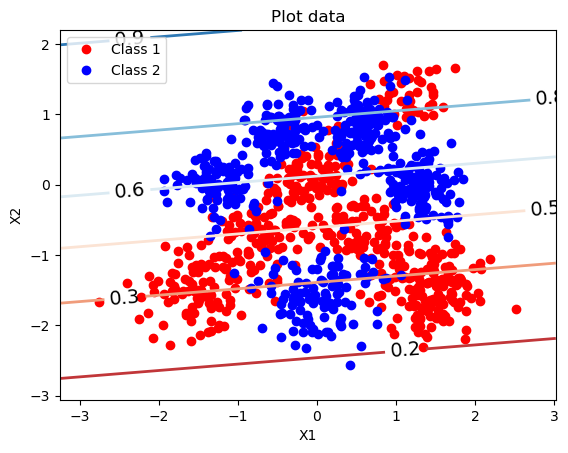
\includegraphics[width=0.3\paperwidth]{fig4.png}
\par\end{centering}
\caption{Visualisation of the contours of the class predictive probabilities.\label{fig:data_visualisation-1} }
\end{figure}


\section{Exercise e)}

The final average training and test log-likelihoods are shown in Table
\ref{tab:average_ll}. These results indicate that this model
underfits the data. These values around -0.6 implies the model
does not classify. For reference, a random guess with 0.5 probabilities for each 
class yields a log-likelihood of $\ln(0.5) \approx -0.7$.



The 2x2 confusion
matrices on the and test set is shown in Table \ref{tab:confusion_test}.
By analysing this table, we conclude that this model does not
classify well. The accuracy is $\frac{357+352}{357+352+149+142} \approx 70\%$.

\begin{table}
\centering{}%
\begin{minipage}[t]{0.49\columnwidth}%
\begin{center}
\begin{tabular}{c|c}
\textbf{Avg. Train ll} & \textbf{Avg. Test ll}\tabularnewline
\hline 
-0.631 & -0.596\tabularnewline
\hline 
\end{tabular} 
\par\end{center}
\caption{Average training and test log-likelihoods.\label{tab:average_ll}}
%
\end{minipage}%
\begin{minipage}[t]{0.49\columnwidth}%
\begin{center}
\begin{tabular}{cc|c|c}
 & \multicolumn{1}{c}{} & \multicolumn{1}{c}{$\hat{y}$} & \tabularnewline
 &  & 0 & 1\tabularnewline
\cline{2-4} 
$y$ & 0 & 357 & 149\tabularnewline
\cline{2-4} 
 & 1 & 142 & 352\tabularnewline
\cline{2-4} 
\end{tabular} 
\par\end{center}
\caption{Confusion matrix on the test set.\label{tab:confusion_test}}
%
\end{minipage}
\end{table}


\section{Exercise f)}

We now expand the inputs through a set of Gaussian radial basis functions
centred on the training datapoints. We consider widths $l=\{0.01,0.1,1\}$
for the basis functions. We fix the learning rate parameter to be
$\eta=\{2\times10^{-3},5\times10^{-3},10^{-4}\}$ for each $l=\{0.01,0.1,1\}$, respectively.
Figure \ref{fig:contours_l} displays the visualisation of the contours
of the resulting class predictive probabilities on top of the data
for each choice of $l=\{0.01,0.1,1\}$.
\begin{figure}
\begin{centering}
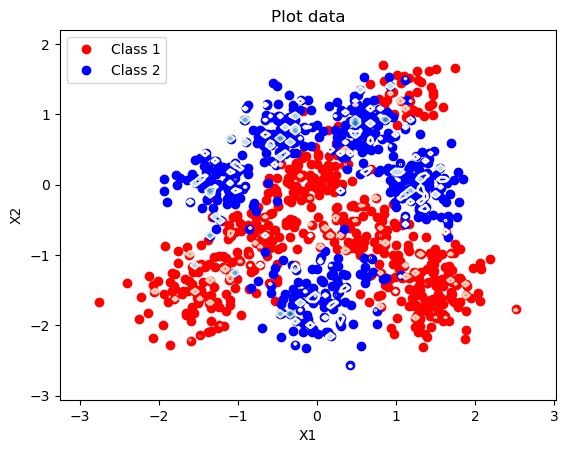
\includegraphics[width=0.32\textwidth]{fig6.png}\hspace{0.15cm}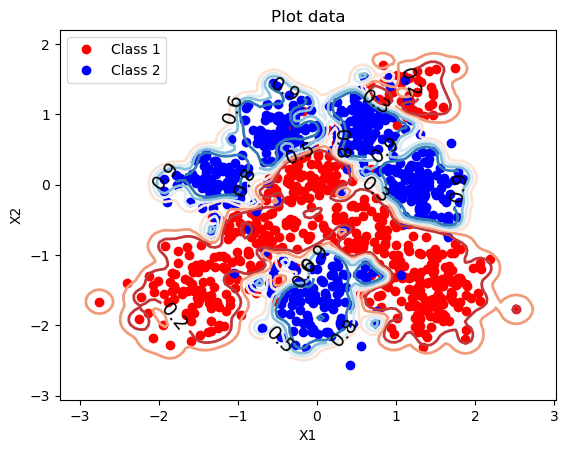
\includegraphics[width=0.32\textwidth]{fig7.png}\hspace{0.15cm}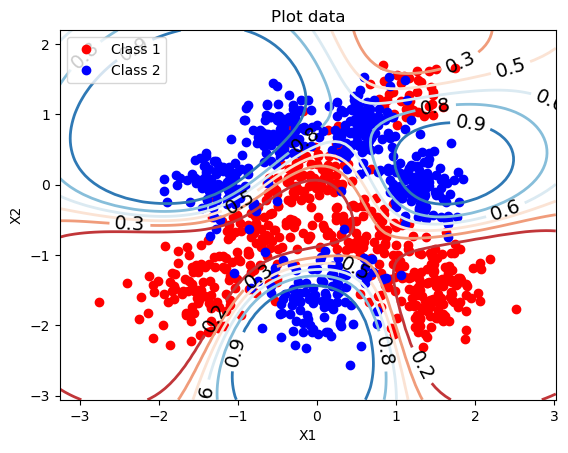
\includegraphics[width=0.32\textwidth]{fig8.png}
\par\end{centering}
\caption{Visualisation of the contours of the class predictive probabilities
for $l=0.01$ (left), $l=0.1$ (middle), $l=1$ (right).\label{fig:contours_l} }
\end{figure}


\section{Exercise g)}

The final final training and test log-likelihoods per datapoint obtained
for each setting of $l=\{0.01,0.1,1\}$ are shown in tables \ref{tab:avg_ll_l_001},
\ref{tab:avg_ll_l_01} and \ref{tab:avg_ll_l_1}. These results indicate
that $l = 0.1$ provides the best classfication among the values of $l$,
since it has the highest value of log-likelihood. $e^{-0.197} = 0.821$
implies that it has a probability of $82\%$ to classify correctly.
$l = 1$ provides a slightly poorer classification. However, $l = 0.01$
lacks at generalization. The test set has a log-likelihood close to the 
theoretical minimum value $\ln(0.5) = -0.69$. 


The 2 \texttimes{} 2 confusion matrices for the three models
trained with $l=\{0.01,0.1,1\}$ are show in tables \ref{tab:conf_l_001},
\ref{tab:conf_l_01} and \ref{tab:conf_l_1}. After analysing these
matrices, we can say that $l = 0.1$ has the highest accuracy.


When we compare these results to those
obtained using the original inputs we conclude that using 
Gaussian Radial Basis functions can obviously enhance 
the performance of the classifier. However, the parameters 
should be chosen with consideration, or it could also perform worse.

\begin{table}
\centering{}%
\begin{minipage}[t]{0.3\textwidth}%
\begin{center}
\begin{tabular}{c|c}
\textbf{Avg. Train ll} & \textbf{Avg. Test ll}\tabularnewline
\hline 
-0.390 & -0.674\tabularnewline
\hline 
\end{tabular}\caption{Results for $l=0.01$\label{tab:avg_ll_l_001}}
\par\end{center}%
\end{minipage}\hspace{0.5cm}%
\begin{minipage}[t]{0.3\textwidth}%
\begin{center}
\begin{tabular}{c|c}
\textbf{Avg. Train ll} & \textbf{Avg. Test ll}\tabularnewline
\hline 
-0.120 & -0.197\tabularnewline
\hline 
\end{tabular}\caption{Results for $l=0.1$\label{tab:avg_ll_l_01}}
\par\end{center}%
\end{minipage}\hspace{0.5cm}%
\begin{minipage}[t]{0.3\textwidth}%
\begin{center}
\begin{tabular}{c|c}
\textbf{Avg. Train ll} & \textbf{Avg. Test ll}\tabularnewline
\hline 
-0.259 & -0.251\tabularnewline
\hline 
\end{tabular}\caption{Results for $l=1$\label{tab:avg_ll_l_1}}
\par\end{center}%
\end{minipage}
\end{table}

\begin{table}
\centering{}%
\begin{minipage}[t]{0.33\textwidth}%
\begin{center}
\begin{tabular}{cc|c|c}
 & \multicolumn{1}{c}{} & \multicolumn{1}{c}{$\hat{y}$} & \tabularnewline
 &  & 0 & 1\tabularnewline
\cline{2-4} 
$y$ & 0 & 476 & 30\tabularnewline
\cline{2-4} 
 & 1 & 129 & 365\tabularnewline
\cline{2-4} 
\end{tabular} 
\par\end{center}
\caption{Conf. matrix $l=0.01$.\label{tab:conf_l_001}}
%
\end{minipage}%
\begin{minipage}[t]{0.33\textwidth}%
\begin{center}
\begin{tabular}{cc|c|c}
 & \multicolumn{1}{c}{} & \multicolumn{1}{c}{$\hat{y}$} & \tabularnewline
 &  & 0 & 1\tabularnewline
\cline{2-4} 
$y$ & 0 & 481 & 25\tabularnewline
\cline{2-4} 
 & 1 & 31 & 463\tabularnewline
\cline{2-4} 
\end{tabular} 
\par\end{center}
\caption{Conf. matrix $l=0.1$.\label{tab:conf_l_01}}
%
\end{minipage}%
\begin{minipage}[t]{0.33\textwidth}%
\begin{center}
\begin{tabular}{cc|c|c}
 & \multicolumn{1}{c}{} & \multicolumn{1}{c}{$\hat{y}$} & \tabularnewline
 &  & 0 & 1\tabularnewline
\cline{2-4} 
$y$ & 0 & 451 & 55\tabularnewline
\cline{2-4} 
 & 1 & 44 & 450\tabularnewline
\cline{2-4} 
\end{tabular} 
\par\end{center}
\caption{Conf. matrix $l=1$.\label{tab:conf_l_1}}
%
\end{minipage}
\end{table}


\section{Conclusion}
In this lab, we successfully designed 
a binary classifier using MLE. 
Our experiments confirm that while linear model
fails to adequately model complex, 
intertwined datasets. Which is evidenced by a 
low average log-likelihood and 
significant misclassifications shown by the
confusion matrix. By introducing Gaussian 
RBF, we achieved a substantial 
performance gain, increasing test accuracy to 82\%. 
However, we also observed that hyperparameter 
sensitivity, mainly including learning rate 
and RBF bandwidth, plays a critical role in 
training stability. 
Future work could involve automated 
hyperparameter tuning to further 
refine the decision boundary.

\end{document}
